% ++++++++++++++++++++++++++++++++++++++++
% Don't modify this section unless you know what you're doing!
\documentclass[letterpaper,12pt]{article}
\usepackage{tabularx} % extra features for tabular environment
\usepackage{amsmath}  % improve math presentation
\usepackage{graphicx} % takes care of graphic including machinery
\usepackage[margin=0.75in,letterpaper]{geometry} % decreases margins
\usepackage{cite} % takes care of citations
\usepackage[final]{hyperref} % adds hyper links inside the generated pdf file
\usepackage{listings}
\usepackage{csvsimple}
\usepackage{verbatim}
\usepackage{float}
\usepackage{graphicx} % Allows including images
\hypersetup{
	colorlinks=true,       % false: boxed links; true: colored links
	linkcolor=black,        % color of internal links
	citecolor=blue,        % color of links to bibliography
	filecolor=magenta,     % color of file links
	urlcolor=blue         
}
%++++++++++++++++++++++++++++++++++++++++
\setlength{\parindent}{0pt}
\setlength\parskip{1em plus 0.1em minus 0.2em}

\begin{document}
\title{%
PyLab - Ohm and Power laws \\
\large PHY224 Lab 1}
\author{Fredrik Dahl Bråten, Pankaj Patil}
\date{\today}
\maketitle
\tableofcontents
\listoffigures
\listoftables

\pagebreak

\section{Exercise 1:  Introduction to fitting methods}

\subsection{Abstract}

Ohm's law explains the relationship between current flowing through a resistor and voltage applied across it.
As per Ohm's law, the current flowing through a resistor is directly proportional to the
voltage applied to its ends. So we have,

$$V = IR$$

Where,
\begin{itemize}
  \item[] $V=$ Voltage
  \item[] $I=$ Current
  \item[] $R=$ Constant of Proportionality (Resistance)
\end{itemize}

In this exercise, using Python modules for data analysis, namely numpy, scipy, we 
verify the Ohm's law. Voltage and Current values are recorded for a known resistor 
and for a Potentiometer using digital multimeters. These recorded values are then
used to arrive at the linear relation and obtain the values of the proportionality constants  between
the voltages and currents. 

The quality of linear fit is obtained by calculating the $\chi^2_{red}$ for the recorded measurements 
for the resistor and Potentiometer. 

The visual analysis of the data is done by plotting the measured data with uncertainty values, along with the linear model
fit graphically, using matplotlib.pyplot Python module.

\subsection{Introduction}

In this exercise we analyze the relationship between current through a circuit element (Resistor or Potentiometer), and the voltage applied across that element. 
With this analysis we establish the Ohm's law which predicts the value of Current, given the value of Resistance and the 
Voltage across the resistor.

The relation we want to verify is $$I = \frac{V}{R}$$

Here we take $V$, the voltage, as independent variable, and $I$, the current as dependent variable. Using the measured data
we use the linear model function $$f(x) = ax + b$$ to fit the data. 

In above expression $x$ is the independent variable which we measure as Voltage, and $f(x)$ is the dependent variable, which is 
the Current.

\subsection{Methods, Materials and Experimental Procedure}

We followed the method described in the lab manual\cite{lab-manual-ex1} to setup the circuit. Setup as shown in circuit
diagram in Figure \ref{setup}, was used to do the measurements.

\begin{figure}[H]
  \centering
  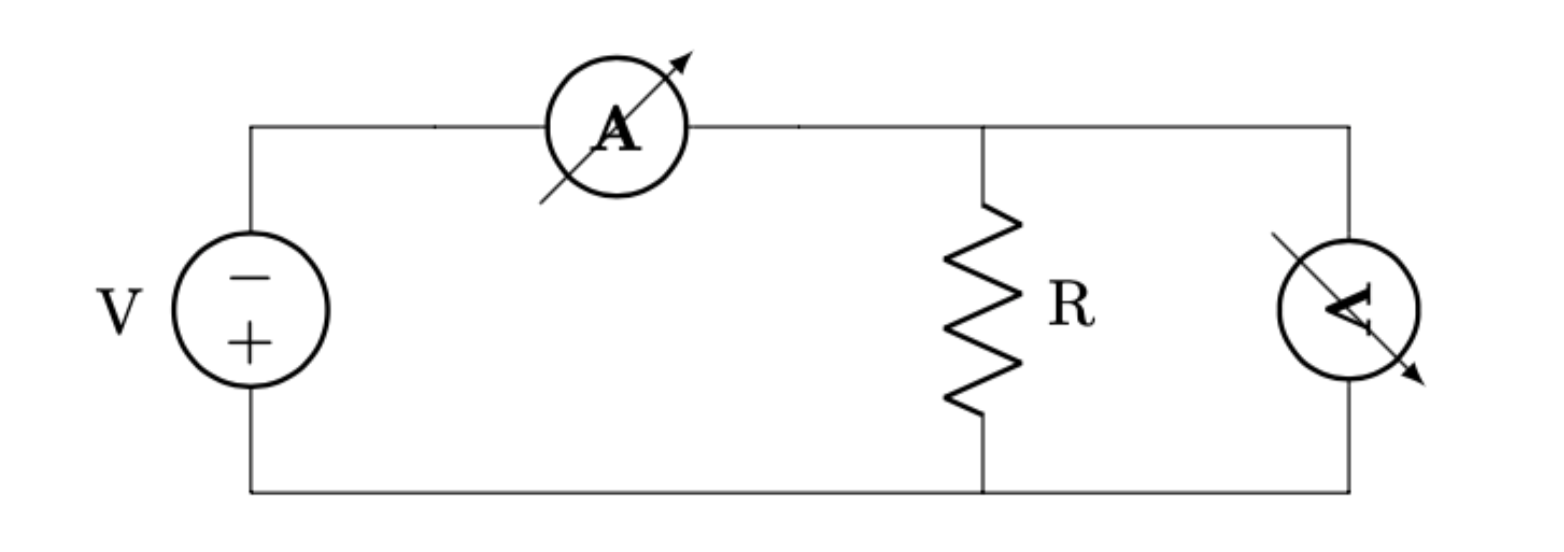
\includegraphics[width=0.9\linewidth]{../Exercise1/lab_1_ex_1_setup.png}    
  \caption{Electrical Circuit Setup}
  \label{setup}
\end{figure}

Measurements were taken for $100 k\Omega$ resistor and for a Potentiometer. Reference values
for 100 $k\Omega$ resistor and Potentiometer were recorded as shown in Table \ref{refdata}. The reference value
for $100 k\Omega$ resistor was computed using the color codes, and that for the Potentiometer 
was recorded using the multimeter.

\begin{table}[H]
  \centering
  \csvautotabular{../Exercise1/reference_resistance.csv}
  \caption{Reference Resistance Values}
  \label{refdata}
\end{table}

For the Potentiometer, we accidentally changed the resistance before noting down the reference value. We chose to
discard the readings taken, and took different set of measurements along with reference resistance without disturbing
the setup the second time.

The uncertainty computation is done using the multimeter accuracy error ($0.75 \%$) and the error in 
precision, which is the fluctuation in last digit of the multimeter ($0.01\ mA$). To account for the other
external factors as described in the lab manual section 4.1\cite{lab-manual-ex1}, we assume additional $2\%$ error in our measurements.

\subsection{Results}

Following the experimental procedures described in previous section, data for Voltage and Current values was recorded for 
$100\ k\Omega$ resistor and Potentiometer in Table \ref{100kdata}, and Table \ref{potentiometerdata} respectively.

The plots of measured current versus voltage for 100 $k\Omega$ and Potentiometer are shown in Figure \ref{100k-curve-fit}
and Figure \ref{potentiometer-curve-fit} respectively.

In both the plots, the linear fit for measured data is drawn using the predicted value of currents by the linear model  parameters
obtained by scipy.optimize.curve\_fit function.



For 100 $k\Omega$ resistor, we get the optimal parameters for model $f(x)= ax+b$ as
$$[a,b] = [0.0102\ 0.0001] \pm [0.0004\ 0.0064]$$
We compute the resistance,
$$R = \frac{1}{a} \pm \Delta a= 98.1500 \pm 0.0004 \ k\Omega$$

For Potentiometer, we get the optimal parameters for model $f(x)= ax+b$ as
$$[a,b] = [0.0638\ 0.0020] \pm [0.0011\ 0.0077]$$
We compute the resistance as,
$$R = \frac{1}{a} \pm \Delta a= 15.6634 \pm 0.0011 \ k\Omega$$

The uncertainty in resistance $R$ is given by quadrature formula
$$R = \frac{1}{a} \implies \Delta R = \Delta a$$

\begin{figure}[H]
  \centering
  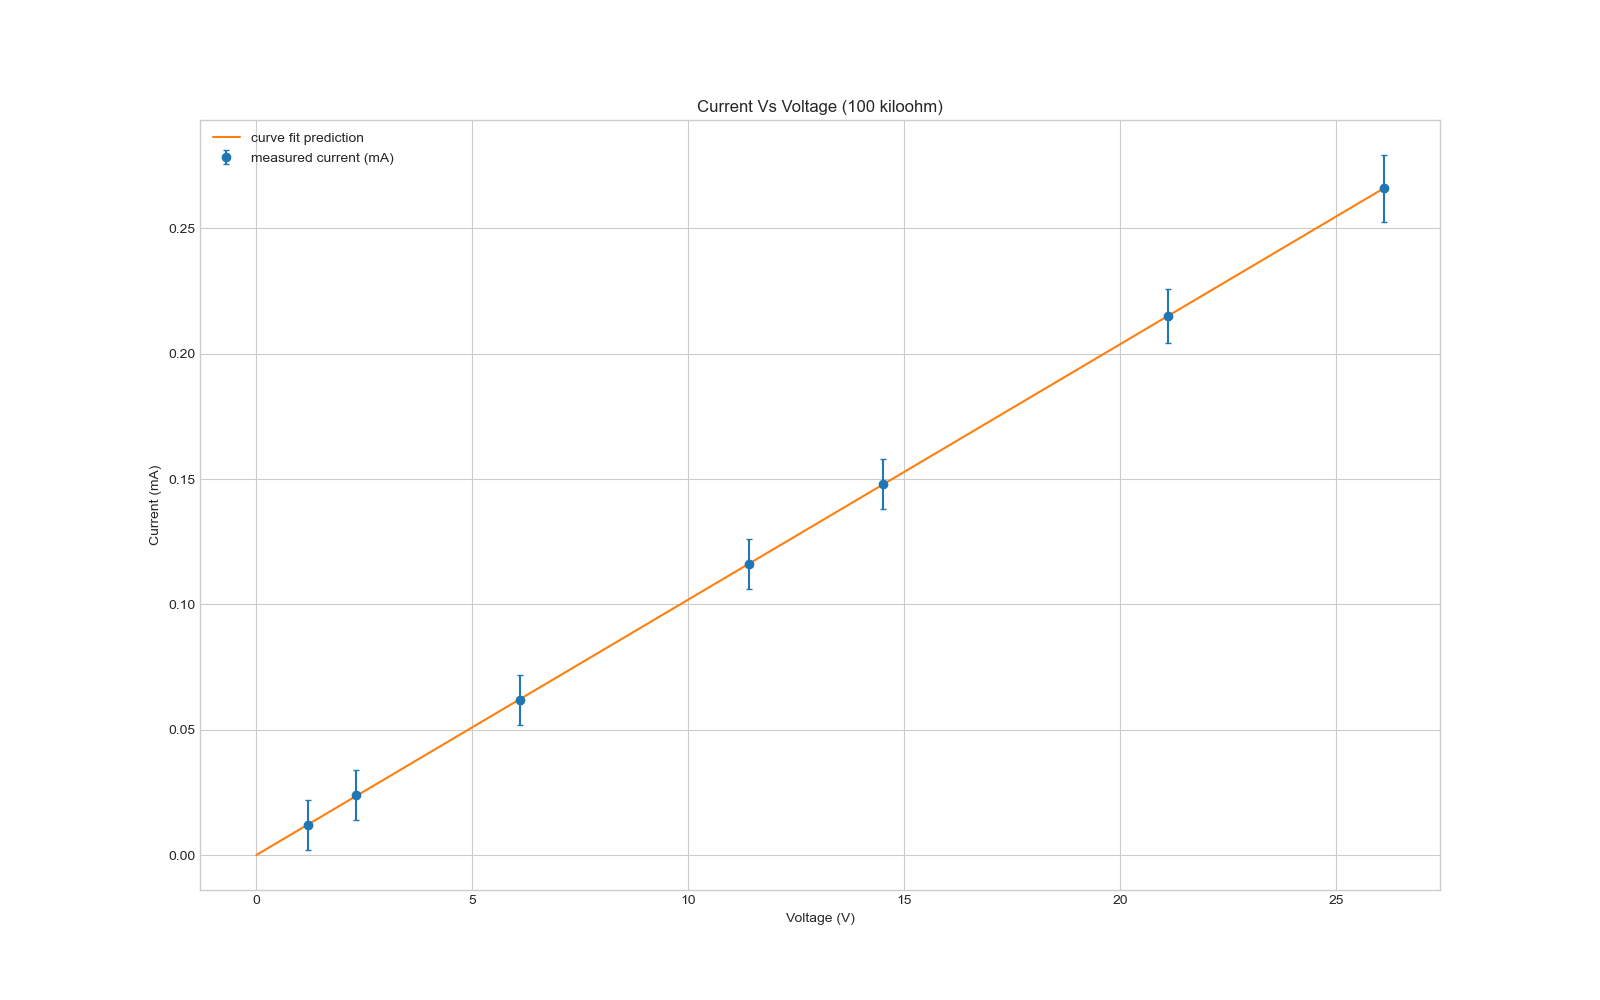
\includegraphics[width=0.95\linewidth]{../Exercise1/lab_1_ex_1_plot_100k.png}   
  \begin{center}
    $f(x) = (0.0102 \pm 0.0004) x + (0.0001 \pm 0.0064),\ \ \ \chi^2_{red} = 0.0009,\ \ \ R = \frac{1}{a}\pm \Delta a = 98.1499 \pm 0.0004 \ k\Omega $
    
    $f(x) = (0.0102 \pm 0.0003) x,\ \ \ \chi^2_{red} = 0.0008,\ \ \ R = \frac{1}{a}\pm \Delta a = 98.1189 \pm 0.0003 \ k\Omega $
    
  \end{center}  
  \caption{100 $k\Omega$ Data Curve Fitting}
  \label{100k-curve-fit}
\end{figure}


\begin{figure}[H]
  \centering
  \includegraphics[width=0.95\linewidth]{../Exercise1/lab_1_ex_1_plot_potentiometer.png}   
  \begin{center}
    $f(x) = (0.0638 \pm 0.0011) x + (0.0020 \pm 0.0011),\ \ \ \chi^2_{red} = 0.0201,\ \ \ R = \frac{1}{a} \pm \Delta a= 15.660 \pm 0.0011  \ k\Omega $
    
    $f(x) = (0.0641 \pm 0.0005) x,\ \ \ \chi^2_{red} = 0.0257,\ \ \ R = \frac{1}{a}\pm \Delta a = 15.660 \pm 0.0005 \ k\Omega $
    
  \end{center}  
  \caption{Potentiometer Data Curve Fitting}
  \label{potentiometer-curve-fit}
\end{figure}

\subsection{Discussion}

In this exercise, the data sets obtained using the measurements were used as is without discarding any data points. As was 
suggested in the manual the data analysis was done for linear models, $f(x) = ax +b$ and $f(x) =  ax$.

The uncertainty calculations are based on error in multimeter accuracy (0.75\%) provided by the manufacturer and error in precision of
the measurement obtained. The error in precision was taken to be fluctuations in last digit of each measurement,  which
we found to be consistent at 0.01 mA. To account for various other factors contributing to error in the measurement
we added 2\% correction factor to the error estimate. The final uncertainty was taken as higher of the three uncertainty
values.

The readings were then fit to linear model using the scipy.optimize.curve\_fit function. In both the cases, namely 100 $k\Omega$
resistor and Potentiometer, the data is plotted along with the model predictions, as shown in Figure \ref{100k-curve-fit} and 
Figure \ref{potentiometer-curve-fit}. We note that for both models and both circuit elements, the predicted graph
passes through the data points error bars nicely. The linear models are more than good fit is evident 
from the fact that in all cases we get low values of $\chi^2_{red}$.

When data is fit to $f(x) = ax + b$, we note that the y-intercept of the line is not zero, although it is a really low value for all the cases. Hence 
for this model the predicted graph does not pass through point (0,0). The reason for non-zero y-intercept can be attributed to
the uncertainties in the measurements. When we force the linear model $f(x) = ax$, the $\chi_{red}^2$ values are little higher, for example,
in Potentiometer case, it is 0.0257 for $f(x) = ax$ against 0.0201 for $f(x) = ax + b$. But in both the cases it is less than 1, giving more than
a good fit. 

The graph lines for both the models are indistinguishable on the plots, in both 100 $k\Omega$ and 
Potentiometer cases. The uncertainty in the measurement of resistance in $f(x) = ax$ is slightly less than the same obtained with $f(x) = ax + b$.

Using both the models the resistance values match with the measured values recorded in Table \ref{refdata}, within
uncertainties of measurements, really well.

The low values of $\chi_{red}^2$ indicate that we have an over-fit model and we needed more readings to do the data analysis. But 
the resistors for electrical circuits are designed to be highly linear and reliable \cite{lab-manual-ex1}, hence we expect to get low values 
for $\chi_{red}^2$. 

\subsection{Conclusions}

In this exercise, we successfully demonstrated the linear relationship between the Voltage across a 
resistor and  the current flowing through it. Using the Python data analysis modules like numpy and scipy we 
were able to obtain optimal parameters for linear model function. The optimal parameters matched within
the uncertainty to the reference values of the resistance we recorded for 100 $k\Omega$ resistor and
Potentiometer. The low values of $\chi_{red}^2$ in both the cases
indicate that we have over-fit model. But as noted in the lab manual\cite{lab-manual-ex1}, resistors
for electrical circuits are designed to be very linear and reliable, hence we expect low values of
$\chi_{red}^2$ for measured data.

\pagebreak

\section{Exercise 3:  Nonlinear fitting methods II}

\subsection{Abstract}

An incandescent lightbulb works by heating a tungsten filament until it glows. 
All matter emits electromagnetic radiation, called thermal radiation, 
when it has a temperature above absolute zero. 
In this report we present how we performed an experiment to compare 
the blackbody power law: $I \propto V^{\frac{3}{5}}$ and the power law for a tungsten wire: 
$I \propto V^{0.5882}$, to the model power laws we estimated from our data: 
measuring voltage and current in a circuit with a lightbulb. 
These theoretical power laws are graphically compared with 
our model power laws. Furthermore, to determine the quality of our models, 
we calculate the $\chi^2_{red}$ values of each model. We also confirmed 
that the theoretical voltage exponent values fell within the uncertainty range 
of our estimated model exponent values. This analysis was done in Python with use 
of the numpy, scipy and matplotlib modules.

\subsection{Introduction}

In this exercise we will model the relationship between voltage and current flowing 
through a circuit with a lightbulb. The corresponding theoretical power law for a 
radiating blackbody is: $I \propto V^{\frac{3}{5}}$, while for a tungsten wire, it is approximately: 
$I \propto V^{0.5882}$. Here I is the measured current, and $V$ is voltage. In our experiment, 
$V$ is the independent variable, and $I$ is the dependent variable. 

We will use two models to approximate the power law from our data: $I = a*V^b$ 
will be our non-linear model, and: $\ln(I) = a*\ln(V)+b$ the linear model for which 
we will fit to our data. $a$ and $b$ are parameters to be adjusted for a best fit, 
while $V$ and $I$ are our measured values of voltage and current. $\ln$ is the natural logarithm.

\subsection{Methods, Materials and Experimental Procedure}

We successfully followed the procedures as described in the exercise3.pdf document\cite{lab-manual-ex2}.

\subsection{Results}
Below in Figure \ref{power-law} and \ref{power-law-log}, we see our data from the experiment plotted as points with 
corresponding error bars. Furthermore, we see the theoretical curves as described in the introduction, 
along with the curves corresponding to our two models best fitted to our data. 
The two models are so similar that it is hard to distinguish them in the plots below.

\begin{figure}[H]
  \centering
  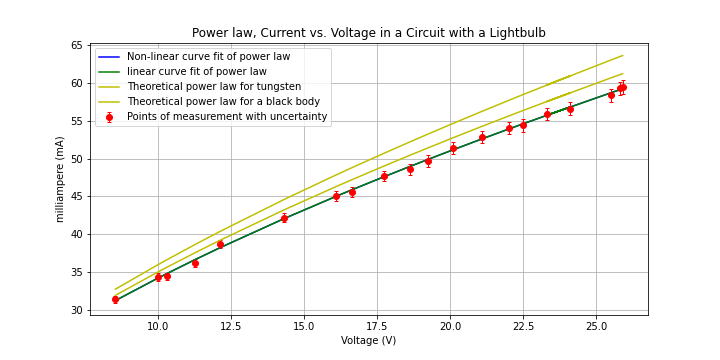
\includegraphics[width=0.95\linewidth]{../Exercise3/Power_law.png}    
  \caption{Points of measurement with corresponding error bars, theoretical power laws for 
  tungsten and a blackbody, along with our two power law models best fitted to our data 
  points.}
  \label{power-law}
\end{figure}

\begin{figure}[H]
  \centering
  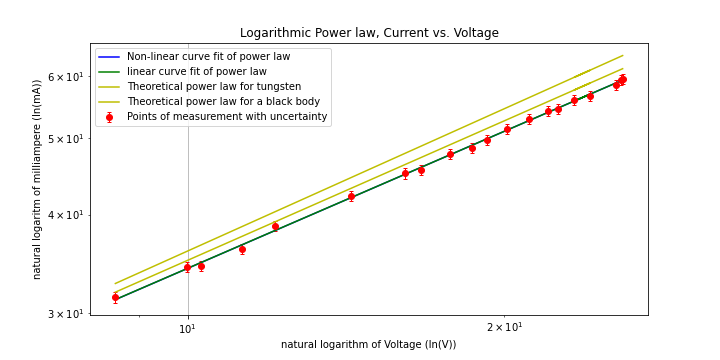
\includegraphics[width=0.95\linewidth]{../Exercise3/Log_Power_law.png}    
  \caption{Equal to Figure \ref{power-law}, though with logarithmic axes.}
  \label{power-law-log}
\end{figure}

The optimal parameters with variance, estimated by the scipy optimize curve fit function, are: 

$[a,b] = [0.57787573\ 2.20117518] \pm [0.00989301\ 0.02841001]$  for the linear model, and: 

$[a,b] = [9.03211882\ 0.57799121] \pm [0.25674234\ 0.00989844]$ for the nonlinear model.

The $\chi^2_{red}$ values for the nonlinear and linear model respectively are 0.19 and 0.19.

The power laws we found between current and voltage, was, with our non-linear model: 

$I(V)= 9.0321 * V ^ {0.5780} $

For our linear model, we found:  

$2.2012 * \exp( 0.5779 * V )$,

Where $V$ is the measured voltage (in volts) and $I$ is current (in milliampere).

\subsection{Discussion}

The uncertainties of the measured current, our dependent variable, 
were initially estimated by picking the maximum uncertainty caused by accuracy and precision. 
The uncertainty of accuracy was caused by the ammeter we used in our experiment. 
The manufacturer of the ammeter writes in its manual that there is an 
estimated measurement uncertainty of $0.75$\% of the value measured by the ammeter. 
The uncertainty of precision was caused by variation over time of the last digit of 
the measured current of the ammeter. The last digit in our experiment was the first 
decimal place with milliampere units, so we estimated an uncertainty due to precision 
of 0.1 milliampere. Our initial estimates of the uncertainty, corresponding to each
 data point in our experiment, was the maximum of the uncertainty due to precision, and accuracy.

However, with these uncertainties our model curves did not pass through 
the error bars of each data point in the experiment. To solve this problem, 
we had to multiply the uncertainty by a factor of 2. The result is shown in 
Figure \ref{power-law} and \ref{power-law-log} in the Results section.

The $\chi^2_{red}$ values calculated for each model, see the Results section, are acceptable values. Thus, the spread (Euclidian distance) between our data points and our two model curves are low. This is good. However, the $\chi^2_{red}$ values are perhaps a bit too small. In our next experiment we will consider gathering more data to increase the $\chi^2_{red}$ values of our models. We were taught in our labs that a $\chi^2_{red}$ value should ideally be approximately between 1 and 10, in experiments such as our own.

As seen in Figure \ref{power-law} and \ref{power-law-log}, both models produce approximately the same curve, which fit our data well. However, the theoretical curves describing the power law, current vs. Voltage, for a tungsten lightbulb and a blackbody, both deviate somewhat from our data points and curves. We have programmed the theoretical curves to only differ from the non-linear model curve, by the value of the Voltage exponent.

The exponents of our two models are very close to the theoretical exponents. 
By the theoretical power laws, with tungsten and blackbody respectively, 
current is proportional to voltage to the power of 0.5882 and $\frac{3}{5} = 0.6$. 
While the nonlinear model approximates an exponent of $0.5778 \pm 0.51$,
while the linear model also approximates an exponent of $0.5779 \pm 0.17$. 
These uncertainties are calculated as the square root of the parameter 
variances of our models returned by the scipy curve fit function. 
Thus, the values of our fitted exponent fall within the range of the blackbody 
values ($\frac{3}{5}=0.6$) and the expected value for tungsten (0.5882), 
with our calculated standard deviation.

These small deviations in model exponents, in comparison to theory exponents, 
causes the theoretical curves to deviate from our model curves.

\subsection{Conclusions}

In this exercise we estimated the power law of a lightbulb in a circuit by measuring current and voltage with uncertainties. We successfully followed the instructions for the experiment written in the exercise3.pdf document without issues. Our results show that both our models return approximately the same estimated power law. However, this power law deviates somewhat from the theoretical power laws for a radiating blackbody and a tungsten wire. We have plotted our data, our model and theoretical curves, and calculated each models $\chi^2_{red}$ values. 

\pagebreak

\appendix

\section{Appendix}

\subsection{Data Tables for Exercise 1}
\begin{table}[H]
  \centering
  \csvautotabular{../Exercise1/100k.csv}
  \caption{Readings of Voltage and Current for 100 $k\Omega$ Resistor}
  \label{100kdata}
\end{table}

\begin{table}[H]
  \centering
  \csvautotabular{../Exercise1/Potentiometer.csv}
  \caption{Readings of Voltage and Current for Potentiometer}
  \label{potentiometerdata}
\end{table}

\subsection{Data Table for Exercise 3}
\begin{table}[H]
  \centering
  \csvautotabular{../Exercise3/Data.csv}
  \caption{Readings of Voltage and Current for Exercise 3}
  \label{ex3data}
\end{table}

\pagebreak

\subsection{Python Code: Exercise 1}

The Python code for this exercise is divided into two files. statslab.py file contains utility methods
which we will be frequently using in this course. lab\_1\_ex\_1\_code.py file contains the code which analyzes
the data for 100 $k\Omega$ resistor and Potentiometer.

\subsubsection{statslab.py}
\noindent\rule{\textwidth}{1pt}
\verbatiminput{../Exercise1/statslab.py}
\noindent\rule{\textwidth}{1pt}

\pagebreak

\subsubsection{lab\_1\_ex\_1\_code.py}
\noindent\rule{\textwidth}{1pt}
\verbatiminput{../Exercise1/lab_1_ex_1_code.py}
\noindent\rule{\textwidth}{1pt}

\pagebreak
\subsubsection{Program Output}
\noindent\rule{\textwidth}{1pt}
\verbatiminput{../Exercise1/output.txt}
\noindent\rule{\textwidth}{1pt}

\pagebreak

\subsection{Python Code: Exercise 3}

The Python code for this exercise is divided into two files. Functions.py file contains utility methods
which we will be frequently using in this course. exercise\_3.py file contains the code which analyzes
the data for this experiment.

\subsubsection{Functions.py}

\noindent\rule{\textwidth}{1pt}
\verbatiminput{../Exercise3/Functions.py}
\noindent\rule{\textwidth}{1pt}

\pagebreak

\subsubsection{exercise\_3.py}
\noindent\rule{\textwidth}{1pt}
\verbatiminput{../Exercise3/exercise_3.py}
\noindent\rule{\textwidth}{1pt}
\pagebreak

\begin{thebibliography}{99}

\bibitem{lab-manual-ex1} Lab Manual - PyLab - Ohm and Power laws - Exerciese 1.
\bibitem{lab-manual-ex2} Lab Manual - PyLab - Ohm and Power laws - Exerciese 3.

\end{thebibliography}

\end{document}
